
\begin{DoxyItemize}
\item \hyperlink{curvefit_fitfun}{F\-I\-T\-F\-U\-N Fit a Function}  
\item \hyperlink{curvefit_gausfit}{G\-A\-U\-S\-F\-I\-T Gaussian Curve Fit}  
\item \hyperlink{curvefit_interp2}{I\-N\-T\-E\-R\-P2 2-\/\-D Interpolation}  
\item \hyperlink{curvefit_interplin1}{I\-N\-T\-E\-R\-P\-L\-I\-N1 Linear 1-\/\-D Interpolation}  
\item \hyperlink{curvefit_poly}{P\-O\-L\-Y Convert Roots To Polynomial Coefficients}  
\item \hyperlink{curvefit_polyder}{P\-O\-L\-Y\-D\-E\-R Polynomial Coefficient Differentiation}  
\item \hyperlink{curvefit_polyfit}{P\-O\-L\-Y\-F\-I\-T Fit Polynomial To Data}  
\item \hyperlink{curvefit_polyint}{P\-O\-L\-Y\-I\-N\-T Polynomial Coefficient Integration}  
\item \hyperlink{curvefit_polyval}{P\-O\-L\-Y\-V\-A\-L Evaluate Polynomial Fit at Selected Points}  
\item \hyperlink{curvefit_roots}{R\-O\-O\-T\-S Find Roots of Polynomial}  
\end{DoxyItemize}\hypertarget{curvefit_fitfun}{}\section{F\-I\-T\-F\-U\-N Fit a Function}\label{curvefit_fitfun}
Section\-: \hyperlink{sec_curvefit}{Optimization and Curve Fitting} \hypertarget{vtkwidgets_vtkxyplotwidget_Usage}{}\subsection{Usage}\label{vtkwidgets_vtkxyplotwidget_Usage}
Fits {\ttfamily n} (non-\/linear) functions of {\ttfamily m} variables using least squares and the Levenberg-\/\-Marquardt algorithm. The general syntax for its usage is \begin{DoxyVerb}  [xopt,yopt] = fitfun(fcn,xinit,y,weights,tol,params...)
\end{DoxyVerb}
 Where {\ttfamily fcn} is the name of the function to be fit, {\ttfamily xinit} is the initial guess for the solution (required), {\ttfamily y} is the right hand side, i.\-e., the vector {\ttfamily y} such that\-: \[ xopt = \arg \min_{x} \|\mathrm{diag}(weights)*(f(x) - y)\|_2^2, \] the output {\ttfamily yopt} is the function {\ttfamily fcn} evaluated at {\ttfamily xopt}. The vector {\ttfamily weights} must be the same size as {\ttfamily y}, and contains the relative weight to assign to an error in each output value. Generally, the ith weight should reflect your confidence in the ith measurement. The parameter {\ttfamily tol} is the tolerance used for convergence. The function {\ttfamily fcn} must return a vector of the same size as {\ttfamily y}, and {\ttfamily params} are passed to {\ttfamily fcn} after the argument {\ttfamily x}, i.\-e., \[ y = fcn(x,param1,param2,...). \] Note that both {\ttfamily x} and {\ttfamily y} (and the output of the function) must all be real variables. Complex variables are not handled yet. \hypertarget{curvefit_gausfit}{}\section{G\-A\-U\-S\-F\-I\-T Gaussian Curve Fit}\label{curvefit_gausfit}
Section\-: \hyperlink{sec_curvefit}{Optimization and Curve Fitting} \hypertarget{vtkwidgets_vtkxyplotwidget_Usage}{}\subsection{Usage}\label{vtkwidgets_vtkxyplotwidget_Usage}
The {\ttfamily gausfit} routine has the following syntax \begin{DoxyVerb}  [mu,sigma,dc,gain,yhat] = gausfit(t,y,w,mug,sigmag,dcg,gaing).
\end{DoxyVerb}
 where the required inputs are 
\begin{DoxyItemize}
\item {\ttfamily t} -\/ the values of the independant variable (e.\-g., time samples)  
\item {\ttfamily y} -\/ the values of the dependant variable (e.\-g., f(t))  
\end{DoxyItemize}The following inputs are all optional, and default values are available for each of them. 
\begin{DoxyItemize}
\item {\ttfamily w} -\/ the weights to use in the fitting (set to ones if omitted)  
\item {\ttfamily mug} -\/ initial estimate of the mean  
\item {\ttfamily sigmag} -\/ initial estimate of the sigma (standard deviation)  
\item {\ttfamily dcg} -\/ initial estimate of the D\-C value  
\item {\ttfamily gaing} -\/ initial estimate of the gain  
\end{DoxyItemize}The fit is of the form {\ttfamily yhat=gain$\ast$exp((t-\/mu).$^\wedge$2/(2$\ast$sigma$^\wedge$2))+dc}. The outputs are 
\begin{DoxyItemize}
\item {\ttfamily mu} -\/ the mean of the fit  
\item {\ttfamily sigma} -\/ the sigma of the fit  
\item {\ttfamily dc} -\/ the dc term of the fit  
\item {\ttfamily gain} -\/ the gain of the gaussian fit  
\item {\ttfamily yhat} -\/ the output samples (the Gaussian fits)  
\end{DoxyItemize}Because the fit is nonlinear, a good initial guess is critical to convergence of the solution. Thus, you can supply initial guesses for each of the parameters using the {\ttfamily mug}, {\ttfamily sigmag}, {\ttfamily dcg}, {\ttfamily gaing} arguments. Any arguments not supplied are estimated using a simple algorithm. In particular, the D\-C value is estimated by taking the minimum value from the vector {\ttfamily y}. The gain is estimated from the range of {\ttfamily y}. The mean and standard deviation are estimated using the first and second order moments of {\ttfamily y}. This function uses {\ttfamily fitfun}. \hypertarget{variables_struct_Example}{}\subsection{Example}\label{variables_struct_Example}
Suppose we want to fit a cycle of a cosine using a Gaussian shape.


\begin{DoxyVerbInclude}
--> t = linspace(-pi,pi); 
--> y = cos(t);
--> [mu,sigma,dc,gain,yhat] = gausfit(t,y);
--> plot(t,y,'rx',t,yhat,'g-');
\end{DoxyVerbInclude}


Which results in the following plot  
\begin{DoxyImage}
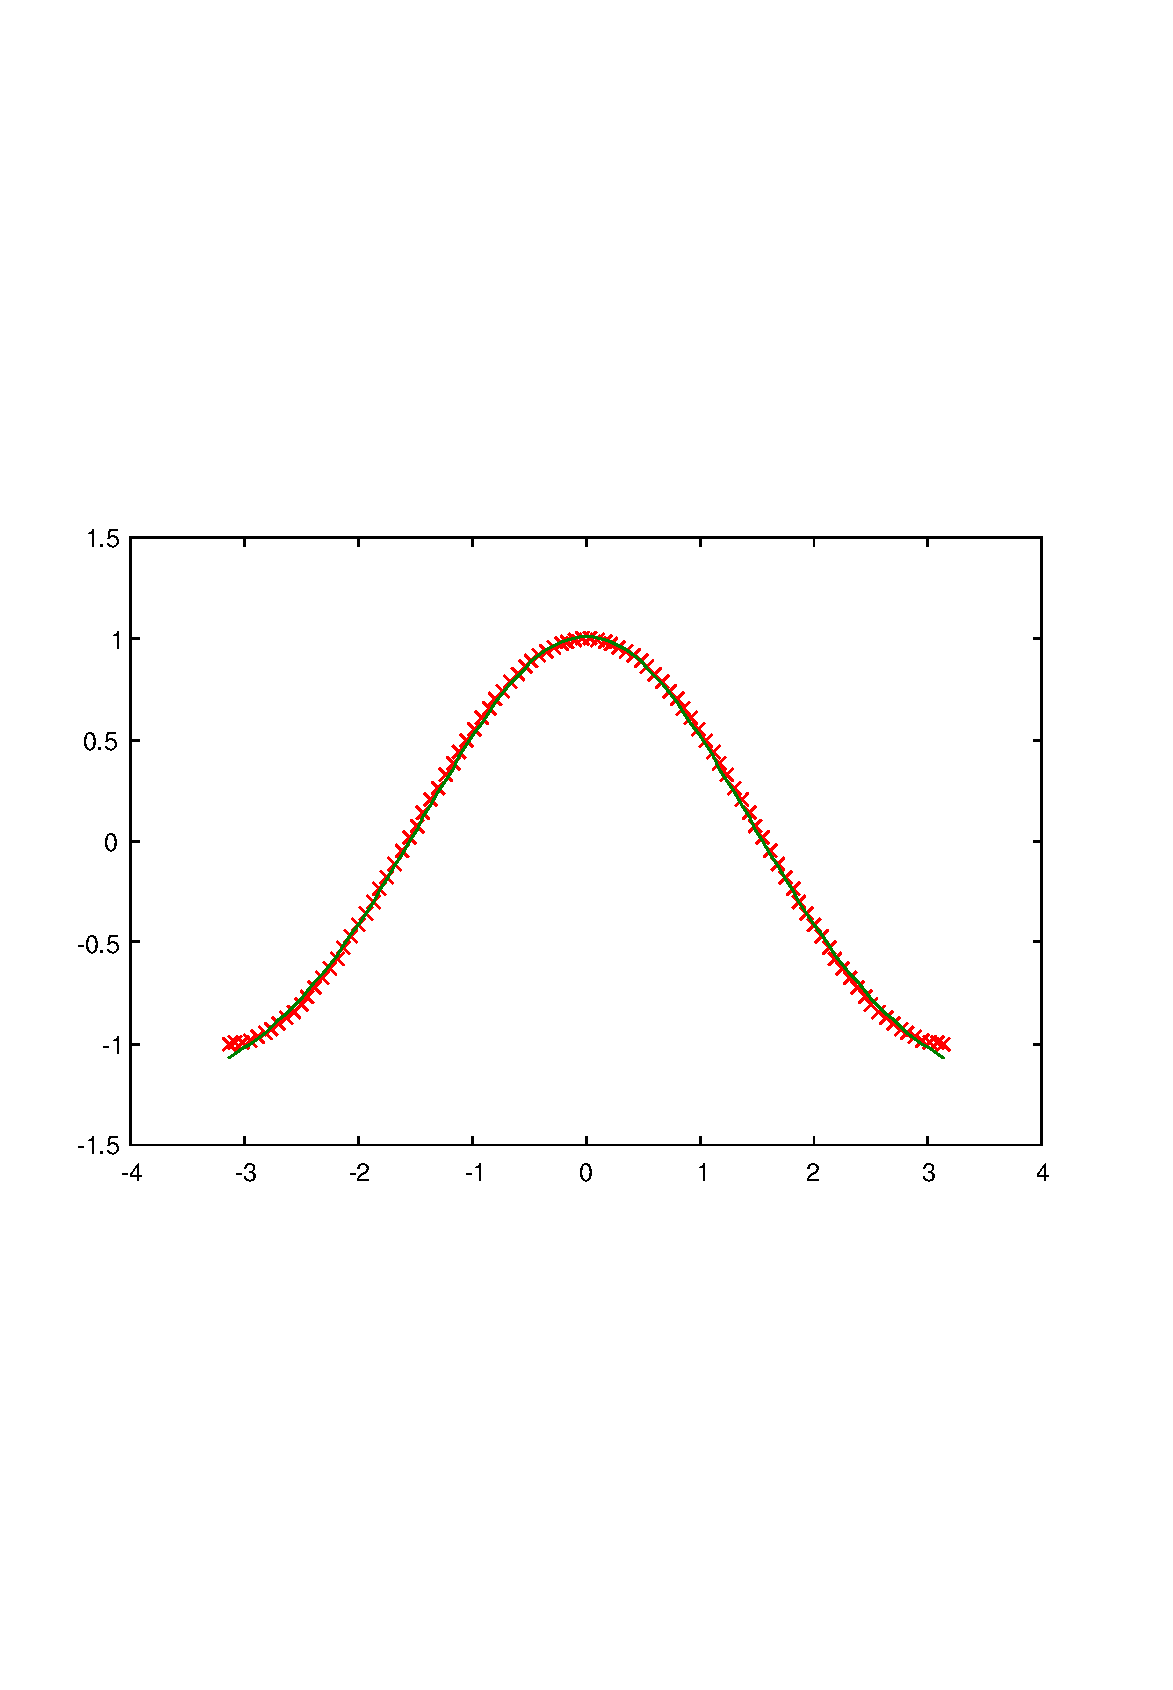
\includegraphics[width=12cm]{gausfit1}
\caption{gausfit1}
\end{DoxyImage}
 \hypertarget{curvefit_interp2}{}\section{I\-N\-T\-E\-R\-P2 2-\/\-D Interpolation}\label{curvefit_interp2}
Section\-: \hyperlink{sec_curvefit}{Optimization and Curve Fitting} \hypertarget{vtkwidgets_vtkxyplotwidget_Usage}{}\subsection{Usage}\label{vtkwidgets_vtkxyplotwidget_Usage}
Given a set of monotonically increasing {\ttfamily x} coordinates and a corresponding set of {\ttfamily y} values, performs simple linear interpolation to a new set of {\ttfamily x} coordinates. The general syntax for its usage is \begin{DoxyVerb}   zi = interp2(z,xi,yi)
\end{DoxyVerb}
 where {\ttfamily xi} and {\ttfamily yi} are vectors of the same length. The output vector {\ttfamily zi} is the same size as the input vector {\ttfamily xi}. For each element of {\ttfamily xi}, the values in {\ttfamily zi} are linearly interpolated by default. Interpolation method can be selected as\-: \begin{DoxyVerb}   zi = interp2(z,xi,yi,method)
\end{DoxyVerb}
 Default interpolation method is {\ttfamily 'linear'}. Other methods are {\ttfamily 'nearest'}, and {\ttfamily 'cubic'}. For values in {\ttfamily xi, yi} that are outside the size of {\ttfamily z}, the default value returned is Na\-N. To change this behavior, you can specify the extrapolation value\-: \begin{DoxyVerb}   zi = interp2(z,xi,yi,method,extrapval)
\end{DoxyVerb}
 The {\ttfamily z} and {\ttfamily xi,yi} vectors must be real, although complex types are allowed for {\ttfamily z}. \hypertarget{curvefit_interplin1}{}\section{I\-N\-T\-E\-R\-P\-L\-I\-N1 Linear 1-\/\-D Interpolation}\label{curvefit_interplin1}
Section\-: \hyperlink{sec_curvefit}{Optimization and Curve Fitting} \hypertarget{vtkwidgets_vtkxyplotwidget_Usage}{}\subsection{Usage}\label{vtkwidgets_vtkxyplotwidget_Usage}
Given a set of monotonically increasing {\ttfamily x} coordinates and a corresponding set of {\ttfamily y} values, performs simple linear interpolation to a new set of {\ttfamily x} coordinates. The general syntax for its usage is \begin{DoxyVerb}   yi = interplin1(x1,y1,xi)
\end{DoxyVerb}
 where {\ttfamily x1} and {\ttfamily y1} are vectors of the same length, and the entries in {\ttfamily x1} are monotoniccally increasing. The output vector {\ttfamily yi} is the same size as the input vector {\ttfamily xi}. For each element of {\ttfamily xi}, the values in {\ttfamily y1} are linearly interpolated. For values in {\ttfamily xi} that are outside the range of {\ttfamily x1} the default value returned is {\ttfamily nan}. To change this behavior, you can specify the extrapolation flag\-: \begin{DoxyVerb}   yi = interplin1(x1,y1,xi,extrapflag)
\end{DoxyVerb}
 Valid options for {\ttfamily extrapflag} are\-: 
\begin{DoxyItemize}
\item {\ttfamily 'nan'} -\/ extrapolated values are tagged with {\ttfamily nan}s  
\item {\ttfamily 'zero'} -\/ extrapolated values are set to zero  
\item {\ttfamily 'endpoint'} -\/ extrapolated values are set to the endpoint values  
\item {\ttfamily 'extrap'} -\/ linear extrapolation is performed  
\end{DoxyItemize}The {\ttfamily x1} and {\ttfamily xi} vectors must be real, although complex types are allowed for {\ttfamily y1}. \hypertarget{variables_struct_Example}{}\subsection{Example}\label{variables_struct_Example}
Here is an example of simple linear interpolation with the different extrapolation modes. We start with a fairly coarse sampling of a cosine.


\begin{DoxyVerbInclude}
--> x = linspace(-pi*7/8,pi*7/8,15);
--> y = cos(x);
--> plot(x,y,'ro');
\end{DoxyVerbInclude}


which is shown here  
\begin{DoxyImage}
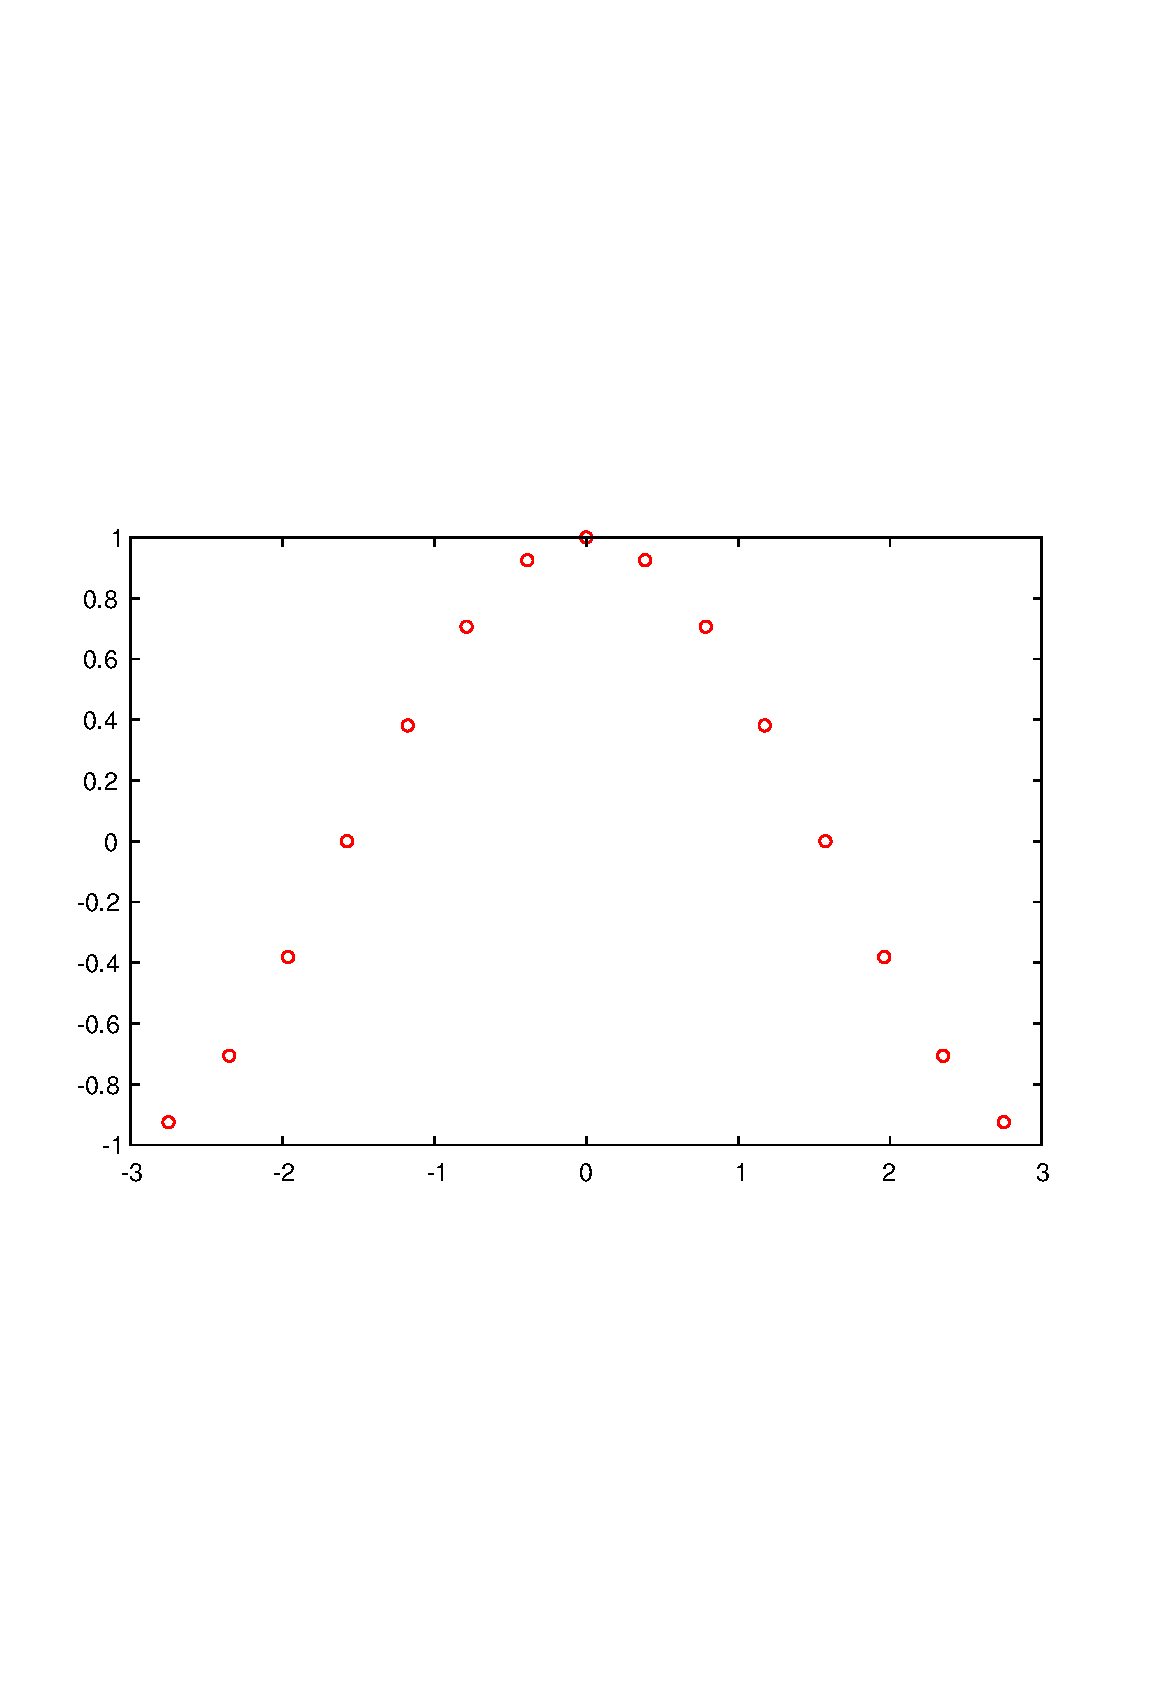
\includegraphics[width=12cm]{interplin1_1}
\caption{interplin1\-\_\-1}
\end{DoxyImage}
 Next, we generate a finer sampling over a slightly broader range (in this case {\ttfamily \mbox{[}-\/pi,pi\mbox{]}}). First, we demonstrate the {\ttfamily 'nan'} extrapolation method


\begin{DoxyVerbInclude}
--> xi = linspace(-4,4,100);
--> yi_nan = interplin1(x,y,xi,'nan');
--> yi_zero = interplin1(x,y,xi,'zero');
--> yi_endpoint = interplin1(x,y,xi,'endpoint');
--> yi_extrap = interplin1(x,y,xi,'extrap');
--> plot(x,y,'ro',xi,yi_nan,'g-x',xi,yi_zero,'g-x',xi,yi_endpoint,'g-x',xi,yi_extrap,'g-x');
\end{DoxyVerbInclude}


which is shown here  
\begin{DoxyImage}
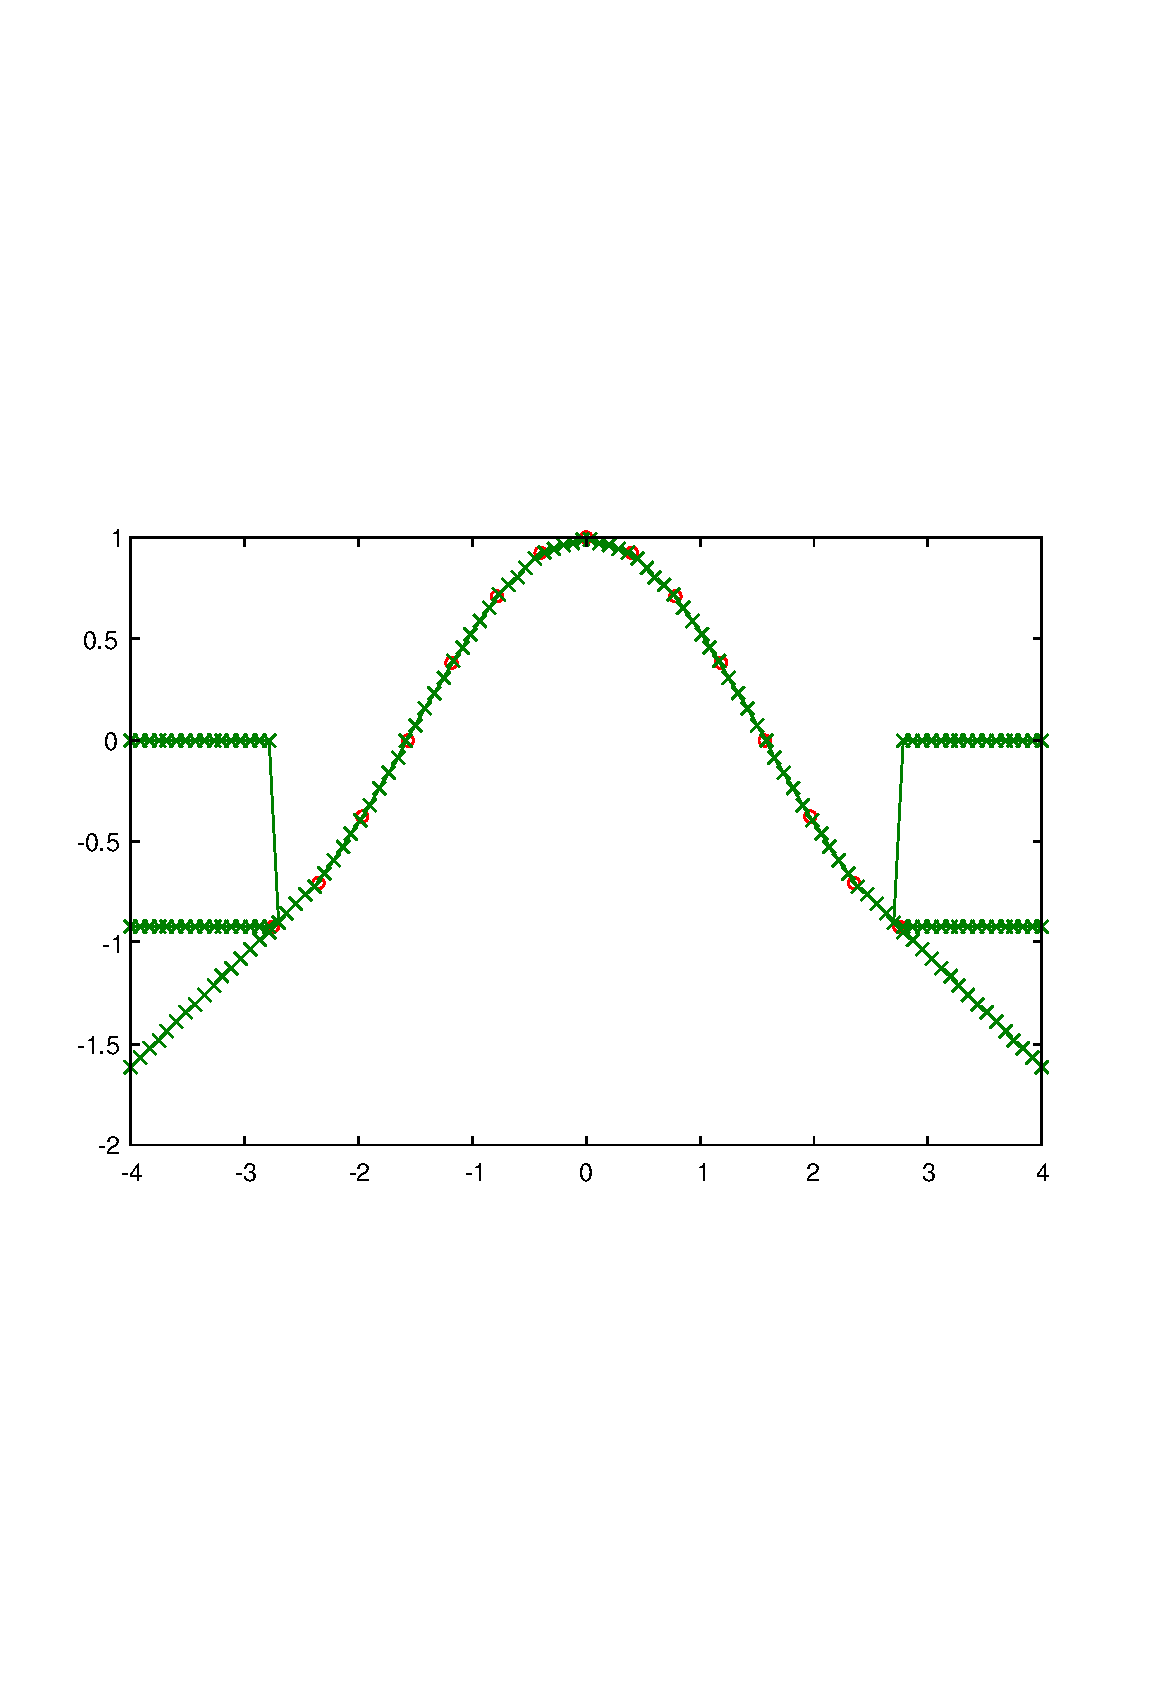
\includegraphics[width=12cm]{interplin1_2}
\caption{interplin1\-\_\-2}
\end{DoxyImage}
 \hypertarget{curvefit_poly}{}\section{P\-O\-L\-Y Convert Roots To Polynomial Coefficients}\label{curvefit_poly}
Section\-: \hyperlink{sec_curvefit}{Optimization and Curve Fitting} \hypertarget{vtkwidgets_vtkxyplotwidget_Usage}{}\subsection{Usage}\label{vtkwidgets_vtkxyplotwidget_Usage}
This function calculates the polynomial coefficients for given roots \begin{DoxyVerb}    p = poly(r)
\end{DoxyVerb}
 when {\ttfamily r} is a vector, is a vector whose elements are the coefficients of the polynomial whose roots are the elements of {\ttfamily r}. Alternately, you can provide a matrix \begin{DoxyVerb}    p = poly(A)
\end{DoxyVerb}
 when {\ttfamily A} is an {\ttfamily N x N} square matrix, is a row vector with {\ttfamily N+1} elements which are the coefficients of the characteristic polynomial, {\ttfamily det(lambda$\ast$eye(size(\-A))-\/\-A)}.

Contributed by Paulo Xavier Candeias under G\-P\-L. \hypertarget{variables_struct_Example}{}\subsection{Example}\label{variables_struct_Example}
Here are some examples of the use of {\ttfamily poly}


\begin{DoxyVerbInclude}
--> A = [1,2,3;4,5,6;7,8,0]

A = 
 1 2 3 
 4 5 6 
 7 8 0 

--> p = poly(A)

p = 
    1.0000   -6.0000  -72.0000  -27.0000 

--> r = roots(p)

r = 
   12.1229 
   -5.7345 
   -0.3884 
\end{DoxyVerbInclude}
 \hypertarget{curvefit_polyder}{}\section{P\-O\-L\-Y\-D\-E\-R Polynomial Coefficient Differentiation}\label{curvefit_polyder}
Section\-: \hyperlink{sec_curvefit}{Optimization and Curve Fitting} \hypertarget{vtkwidgets_vtkxyplotwidget_Usage}{}\subsection{Usage}\label{vtkwidgets_vtkxyplotwidget_Usage}
The {\ttfamily polyder} function returns the polynomial coefficients resulting from differentiation of polynomial {\ttfamily p}. The syntax for its use is either \begin{DoxyVerb} pder = polyder(p)
\end{DoxyVerb}
 for the derivitave of polynomial p, or \begin{DoxyVerb} convp1p2der = polyder(p1,p2)
\end{DoxyVerb}
 for the derivitave of polynomial conv(p1,p2), or still \begin{DoxyVerb} [nder,dder] = polyder(n,d)
\end{DoxyVerb}
 for the derivative of polynomial {\ttfamily n/d} ({\ttfamily nder} is the numerator and {\ttfamily dder} is the denominator). In all cases the polynomial coefficients are assumed to be in decreasing degree. Contributed by Paulo Xavier Candeias under G\-P\-L \hypertarget{variables_struct_Example}{}\subsection{Example}\label{variables_struct_Example}
Here are some examples of the use of {\ttfamily polyder}


\begin{DoxyVerbInclude}
--> polyder([2,3,4])

ans = 
 4 3 
\end{DoxyVerbInclude}



\begin{DoxyVerbInclude}
--> polyder([2,3,4],7)

ans = 
 28 21 
\end{DoxyVerbInclude}



\begin{DoxyVerbInclude}
--> [n,d] = polyder([2,3,4],5)
n = 
 -20 -15 

d = 
 25 
\end{DoxyVerbInclude}
 \hypertarget{curvefit_polyfit}{}\section{P\-O\-L\-Y\-F\-I\-T Fit Polynomial To Data}\label{curvefit_polyfit}
Section\-: \hyperlink{sec_curvefit}{Optimization and Curve Fitting} \hypertarget{vtkwidgets_vtkxyplotwidget_Usage}{}\subsection{Usage}\label{vtkwidgets_vtkxyplotwidget_Usage}
The {\ttfamily polyfit} routine has the following syntax \begin{DoxyVerb}  p = polyfit(x,y,n)
\end{DoxyVerb}
 where {\ttfamily x} and {\ttfamily y} are vectors of the same size, and {\ttfamily n} is the degree of the approximating polynomial. The resulting vector {\ttfamily p} forms the coefficients of the optimal polynomial (in descending degree) that fit {\ttfamily y} with {\ttfamily x}. \hypertarget{transforms_svd_Function}{}\subsection{Internals}\label{transforms_svd_Function}
The {\ttfamily polyfit} routine finds the approximating polynomial \[ p(x) = p_1 x^n + p_2 x^{n-1} + \dots + p_n x + p_{n+1} \] such that \[ \sum_{i} (p(x_i) - y_i)^2 \] is minimized. It does so by forming the Vandermonde matrix and solving the resulting set of equations using the backslash operator. Note that the Vandermonde matrix can become poorly conditioned with large {\ttfamily n} quite rapidly. \hypertarget{variables_struct_Example}{}\subsection{Example}\label{variables_struct_Example}
A classic example from Edwards and Penny, consider the problem of approximating a sinusoid with a polynomial. We start with a vector of points evenly spaced on the unit interval, along with a vector of the sine of these points.


\begin{DoxyVerbInclude}
--> x = linspace(0,1,20);
--> y = sin(2*pi*x);
--> plot(x,y,'r-')
\end{DoxyVerbInclude}


The resulting plot is shown here  
\begin{DoxyImage}
\includegraphics[width=12cm]{polyfit1}
\caption{polyfit1}
\end{DoxyImage}
 Next, we fit a third degree polynomial to the sine, and use {\ttfamily polyval} to plot it


\begin{DoxyVerbInclude}
--> p = polyfit(x,y,3)

p = 
   21.9170  -32.8756   11.1897   -0.1156 

--> f = polyval(p,x);
--> plot(x,y,'r-',x,f,'ko');
\end{DoxyVerbInclude}


The resulting plot is shown here  
\begin{DoxyImage}
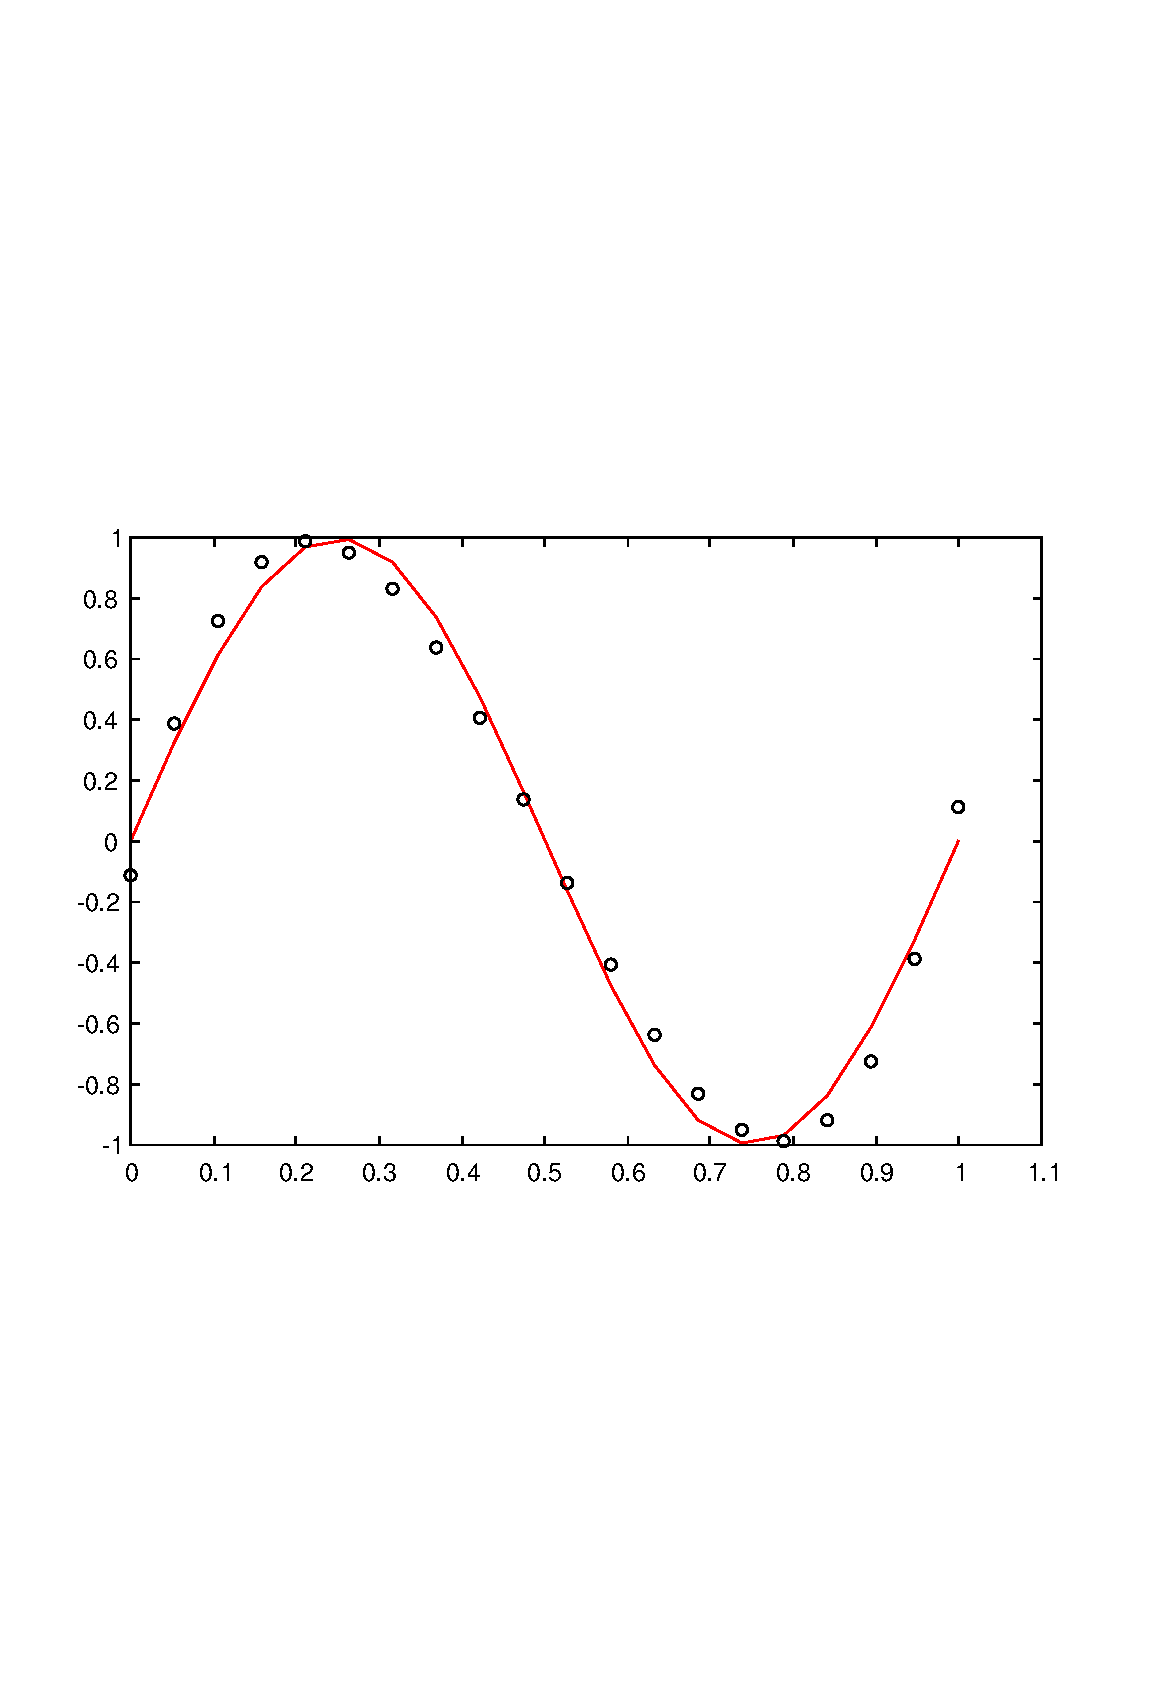
\includegraphics[width=12cm]{polyfit2}
\caption{polyfit2}
\end{DoxyImage}
 Increasing the order improves the fit, as


\begin{DoxyVerbInclude}
--> p = polyfit(x,y,11)

p = 

 Columns 1 to 7

   12.4644  -68.5541  130.0555  -71.0940  -38.2814  -14.1222   85.1018 

 Columns 8 to 12

   -0.5642  -41.2861   -0.0029    6.2832   -0.0000 

--> f = polyval(p,x);
--> plot(x,y,'r-',x,f,'ko');
\end{DoxyVerbInclude}


The resulting plot is shown here  
\begin{DoxyImage}
\includegraphics[width=12cm]{polyfit3}
\caption{polyfit3}
\end{DoxyImage}
 \hypertarget{curvefit_polyint}{}\section{P\-O\-L\-Y\-I\-N\-T Polynomial Coefficient Integration}\label{curvefit_polyint}
Section\-: \hyperlink{sec_curvefit}{Optimization and Curve Fitting} \hypertarget{vtkwidgets_vtkxyplotwidget_Usage}{}\subsection{Usage}\label{vtkwidgets_vtkxyplotwidget_Usage}
The polyint function returns the polynomial coefficients resulting from integration of polynomial p. The syntax for its use is either \begin{DoxyVerb} pint = polyint(p,k)
\end{DoxyVerb}
 or, for a default {\ttfamily k = 0}, \begin{DoxyVerb} pint = polyint(p);
\end{DoxyVerb}
 where {\ttfamily p} is a vector of polynomial coefficients assumed to be in decreasing degree and {\ttfamily k} is the integration constant. Contributed by Paulo Xavier Candeias under G\-P\-L \hypertarget{variables_struct_Example}{}\subsection{Example}\label{variables_struct_Example}
Here is are some examples of the use of {\ttfamily polyint}.


\begin{DoxyVerbInclude}
--> polyint([2,3,4])

ans = 
    0.6667    1.5000    4.0000         0 
\end{DoxyVerbInclude}


And


\begin{DoxyVerbInclude}
--> polyint([2,3,4],5)

ans = 
    0.6667    1.5000    4.0000    5.0000 
\end{DoxyVerbInclude}
 \hypertarget{curvefit_polyval}{}\section{P\-O\-L\-Y\-V\-A\-L Evaluate Polynomial Fit at Selected Points}\label{curvefit_polyval}
Section\-: \hyperlink{sec_curvefit}{Optimization and Curve Fitting} \hypertarget{vtkwidgets_vtkxyplotwidget_Usage}{}\subsection{Usage}\label{vtkwidgets_vtkxyplotwidget_Usage}
The {\ttfamily polyval} routine has the following syntax \begin{DoxyVerb}  y = polyval(p,x)
\end{DoxyVerb}
 where {\ttfamily p} is a vector of polynomial coefficients, in decreasing degree (as generated by {\ttfamily polyfit}, for example). If {\ttfamily x} is a matrix, the polynomial is evaluated in the matrix sense (in which case {\ttfamily x} must be square). \hypertarget{transforms_svd_Function}{}\subsection{Internals}\label{transforms_svd_Function}
The polynomial is evaluated using a recursion method. If the polynomial is \[ p(x) = p_1 x^n + p_2 x^{n-1} + \dots + p_n x + p_{n+1} \] then the calculation is performed as \[ p(x) = ((p_1) x + p_2) x + p_3 \] \hypertarget{variables_struct_Example}{}\subsection{Example}\label{variables_struct_Example}
Here is a plot of {\ttfamily x$^\wedge$3} generated using polyval


\begin{DoxyVerbInclude}
--> p = [1 0 0 0]

p = 
 1 0 0 0 

--> x = linspace(-1,1);
--> y = polyval(p,x);
--> plot(x,y,'r-')
\end{DoxyVerbInclude}


Here is the resulting plot  
\begin{DoxyImage}
\includegraphics[width=12cm]{polyval1}
\caption{polyval1}
\end{DoxyImage}
 \hypertarget{curvefit_roots}{}\section{R\-O\-O\-T\-S Find Roots of Polynomial}\label{curvefit_roots}
Section\-: \hyperlink{sec_curvefit}{Optimization and Curve Fitting} \hypertarget{vtkwidgets_vtkxyplotwidget_Usage}{}\subsection{Usage}\label{vtkwidgets_vtkxyplotwidget_Usage}
The {\ttfamily roots} routine will return a column vector containing the roots of a polynomial. The general syntax is \begin{DoxyVerb}   z = roots(p)
\end{DoxyVerb}
 where {\ttfamily p} is a vector containing the coefficients of the polynomial ordered in descending powers. \hypertarget{transforms_svd_Function}{}\subsection{Internals}\label{transforms_svd_Function}
Given a vector \[ [p_1, p_2, \dots p_n] \] which describes a polynomial \[ p_1 x^{n-1} + p_2 x^{n-2} + \dots + p_n \] we construct the companion matrix (which has a characteristic polynomial matching the polynomial described by {\ttfamily p}), and then find the eigenvalues of it (which are the roots of its characteristic polynomial), and which are also the roots of the polynomial of interest. This technique for finding the roots is described in the help page for {\ttfamily roots} on the Mathworks website. \hypertarget{variables_struct_Example}{}\subsection{Example}\label{variables_struct_Example}
Here is an example of finding the roots to the polynomial \[ x^3 - 6x^2 - 72x - 27 \]


\begin{DoxyVerbInclude}
--> roots([1 -6 -72 -27])

ans = 
   12.1229 
   -5.7345 
   -0.3884 
\end{DoxyVerbInclude}
 